\section{Introduction}
Edward Condon in 1928~\cite{Condon} made with surprisingly little justification the approximation that the electronic transition dipole did not depend on the nuclear position at all.  That approximation has stood in great stead until recently its effects, particularly in dynamic spectroscopy, have become particularly clear.

There are no doubt many more, but among the recent work include invoking a nontrivial transition dipole to explain graphene's anomalous Raman spectrum ~\cite{hellerGraphene}.  Furthermore, recent calculations also predict a highly noticeable transition dipole moment in photosynthetic systems~\cite{photosyntheticKappa}.  There is also most probably a noticeable effect in some electron-transfer systems of a varying transition dipole moment~\cite{MavrosNonCondon}.  Lastly, the introduction of a linear variation in transition dipole, completely broke a proposed detection scheme for electronic versus vibrational coherence.

Thus, as more and more scholarship begins to make clear the importance of variation of the transition dipole to the field of dynamic spectroscopy, it would seem to be eminently useful to have a tool to measure these variations.  While experiments can infer the presence of a nontrivial transition dipole, we believe it is important to work towards an experiment which definitively can determine the structure of a transition dipole moment.

\section{System Setup}
For our purposes we construct the simplest system for which transition dipole variation can affect its spectra: a vibrational monomer with a ground electronic state $\ket{g}$ and an excited electronic state $\ket{e}$ with a different harmonic vibration in both the ground and excited state such that the Hamiltonian looks like this:
\begin{align}
	H_0 &=  \sum_n \hbar \omega_{\gamma}  \left(n + \frac{1}{2} \right)  \ket{n_{\gamma}}\ket{g}\bra{g} \bra{n_{\gamma}} \\
   &+ \sum_m \left(  \hbar \omega_{\epsilon}  \left(m + \frac{1}{2} \right) + \omega_e \right)  \ket{m_{\epsilon}} \ket{e}\bra{e} \bra{m_{\epsilon}}
\end{align}
With the Greek indices corresponding to the vibrational states and the roman indices corresponding to the electronic states.  We give this system an electronic transition dipole:
\begin{align}
	\hat{\mu}(x) &= \mu (x)  \left( \ket{e}\bra{g} + \ket{g} \bra{e} \right)
\end{align}
Where we put all the nuclear variation of the transition dipole moment into the function $\mu(x)$.  Considering what a varying transition dipole may look like, we construct the simplest possible variation: a linear-varying moment, which one can transform into ladder operators for easier calculation:
\begin{align}
	\mu(x) &= \mu_0 \left[ 1 + c \left( \hat{a}_{\gamma} + \hat{a}_{\gamma}^{\dagger}\right)  \right]
\end{align}
where $\hat{a}_{\gamma}$ and $\hat{a}_{\gamma}^{\dagger}$ are ladder operators in the ground state vibrational potential.  One can imagine a more general form of the transition dipole for more than just linear variation:
\begin{align}
	\mu(x) &= \mu_0 \sum_{i=0} \kappa_i x^i \\
	&= \mu_0 \sum_{i=0} c_i \left( \hat{a} + \hat{a}^{\dagger}\right)^i
\end{align}
but we will concerns ourselves exclusively with the linear variation here.  Depending on the context, it can be useful to transition dipole  of the transition dipole as more of a vibrational matrix element:
\begin{align}
	\mu_{a,b} = \bra{a_{\gamma}} \mu(x) \ket{b_{\gamma}}
\end{align}
This equation shows that a nonzero $c$ will cause an application of $ \mu_{a,b}$ to deform the wavefunction, but how?




\section{Mode Heating}
We instead want to work with an object which only exhibits interesting dynamics when there is an interesting transition dipole, like $\ket{\psi_{+,-}(t)}$.

If you imagine hitting our monomer with the positive energy delta-function laser pulse, and then hitting it again immediately after (really at the same time) with the negative energy part of the laser pulse to get a second order perturbation.  Without a transition dipole that varies, one would expect to have a perfect copy of the original vibrational wavepacket, back in the ground electronic state after an instantaneous trip to the excited state.  If, however, there is a variation in the transition dipole, then you would have no longer have a perfect copy, but you would have induced a ground-state vibrational coherence.  Putting this mathematically, we would only expect interesting or novel effects from $\ket{\psi_{+,-}(t)}$, if the transition dipole varies, but it's boring if there is no variation.   Putting it yet another way, a non-trivial transition dipole moment causes a vibrational coherence in the ground state of  $\ket{\psi_{+,-}(t)}$ where there would be none if the transition dipole moment is constant.

Mathematically, it would look like this assuming a delta-function laser beam at $t=0$ and starting in the 0th state:
\begin{align}
	&\ket{\psi_{+,-}(0)} =\\
	&= \mu_0^2 \left[ 1 + c \left( \hat{a}_{\gamma} + \hat{a}_{\gamma}^{\dagger}\right)  \right]\left[ 1 + c^* \left( \hat{a}_{\gamma} + \hat{a}_{\gamma}^{\dagger}\right)  \right] \ket{0_{\gamma}} \ket{g}\\
	&= \mu_0^2 \left[ 1 + \left(c + c^*\right) \left( \hat{a}_{\gamma} + \hat{a}_{\gamma}^{\dagger}\right) + |c|^2 \left( \hat{a}_{\gamma} + \hat{a}_{\gamma}^{\dagger}\right)^2  \right] \ket{0_{\gamma}} \ket{g}\\
	&= \mu_0^2 \left[ (1 + |c|^2) \ket{0_{\gamma}} + \left(c + c^*\right)\ket{1_{\gamma}}  + \sqrt{2}|c|^2 \ket{2_{\gamma}} \right]  \ket{g}
\end{align}
So for the case of a delta function pulse, the wavefunction is either trivially the same ground state if the transition dipole is constant ($c=0$) or it can be a vibrational coherence for nonzero $c$.  That vibrational coherence implies that the ground state has heated up; the average vibrational quantum number is now higher.  We set out to find a way to make a signal out of that.

\subsection{ Resonance Raman }
The simplest signal that could be constructed for this would be
\begin{align*}
	E(t) = -i \omega^2 \bra{\psi_0 (t)} \hat{\mu} \ket{\psi_{+,-} (t) }
\end{align*}
but the transition dipole we introduced earlier would mean this is zero as both the bra and ket are in the ground electronic state, and the transition dipole operator is off-diagonal in the electronic basis.  If, however, the vibrational mode is IR-active, it will have a transition dipole that is diagonal in the electronic basis:
\begin{align}
	\hat{\mu}_{IR} &=  d_g\ket{g}\bra{g} \left( \hat{a}_{\gamma}^{\dagger} + \hat{a}_{\gamma} \right) + d_e \ket{e}\bra{e}\left( \hat{a}_{\epsilon}^{\dagger} + \hat{a}_{\epsilon} \right)
\end{align}
which will give us a signal like so:
\begin{align}
	E_{IR}(t) = i\omega^2  \bra{\psi_0(t)} \hat{\mu}_{IR} \ket{\psi_{+, -} (t) }
\end{align}
which due to phase matching will be isotropic.  This is very similar to the phenomenon of resonance Raman~\cite{ResonanceRaman} but we are predicting an additional isotropic signal as opposed to

To generalize this to real pulses, we treat a more general laser pulse perturbation of the form:
\begin{align}
	H'(\tau) = E(\tau) \mu(x) \left( \ket{e}\bra{g} + \ket{g}\bra{e}\right)
\end{align}
and a starting wavefunction of
\begin{align}
	\ket{\psi_0(0)} = \ket{\eta_{\gamma}} \ket{g}
\end{align}
If we consider times $t$ only after the pulse has turned off, and let $\tilde{E}_{\pm}(\omega)$ be the positive and negative frequency parts of the Fourier transform of $E(\tau)$, we get first as the excitation perturbation:
\begin{align*}
	\ket{\psi_+ (t) } &= \sum_{\lambda,k} \tilde{E}_{+}\left(\Omega_{e}^{(k)} - \Omega_{g}^{(\eta)}\right) \mu_{\eta,\lambda} O_{\lambda}^{k} e^{-i\Omega_{e}^{(k)}}\ket{k_{\epsilon}} \ket{e}
\end{align*}
Going forward we define $\Omega_{e}^{(k)} - \Omega_{g}^{(\eta)} = \Delta \Omega_{(\eta)}^{(k)}$
\begin{align*}
	\ket{\psi_+ (t) } &= \sum_{\lambda,k} \tilde{E}_{+}\left(\Delta \Omega_{(\eta)}^{(k)}\right) \mu_{\eta,\lambda} O_{\lambda}^{k} e^{-i\Omega_{e}^{(k)}}\ket{k_{\epsilon}} \ket{e}
\end{align*}
then we bring in the relaxation or negative frequency part of the perturbation and apply again to get:
\begin{align*}
	\ket{\psi_{+, -} (t) } =\\
	 \sum_{\lambda,k, a, b} \tilde{E}_{+} \left(\Delta \Omega_{(\eta)}^{(k)}\right)  \tilde{E}_{-}\left(-\Delta \Omega_{(b)}^{(k)}\right)  \mu_{\eta,\lambda}\mu_{a,b} O_{\lambda}^{k} O_{a}^{k} e^{-i\Omega_{g}^{(b)}} \ket{b_{\gamma}} \ket{g}
\end{align*}

Now we apply the IR transition dipole to the ground state
\begin{align*}
	\hat{\mu}_{IR}\ket{\psi_0 (t) } =&  d_ge^{-i \Omega_{g}^{(\eta )} t}  \left(\sqrt{\eta}\ket{\eta-1_{\gamma}}  + \sqrt{\eta + 1}\ket{\eta+1_{\gamma}}  \right)\ket{g}
\end{align*}
which we then combine together with the perturbed wavefunction to get:


\begin{align*}
	&\frac{1}{\omega_{\gamma}^2d_g}E_{IR}(t) = \\
	&\sqrt{\eta}\sum_{\lambda,k, a} \tilde{E}_{+} \left(\Delta \Omega_{(\eta)}^{(k)}\right)  \tilde{E}_{-}\left(-\Delta \Omega_{(\eta-1)}^{(k)}\right)  \mu_{\eta,\lambda}\mu_{a,\eta-1} \\
	&\times O_{\lambda}^{k} O_{a}^{k} e^{i \omega_{\gamma} t} \\
	&+ \sqrt{\eta+1}\sum_{\lambda,k, a} \tilde{E}_{+} \left(\Delta \Omega_{(\eta)}^{(k)}\right)  \tilde{E}_{-}\left(-\Delta \Omega_{(\eta+1)}^{(k)}\right)  \mu_{\eta,\lambda}\mu_{a,\eta+1} \\
	&\times O_{\lambda}^{k} O_{a}^{k} e^{-i\omega_{\gamma} t}
\end{align*}
if we assume the 0th state initially it gets a little simpler:
\begin{align*}
	&\frac{1}{\omega_{\gamma}^2d_g}E_{IR}(t) = \\
	&\sum_{\lambda,k, a} \tilde{E}_{+} \left(\Delta \Omega_{(0)}^{(k)}\right)  \tilde{E}_{-}\left(-\Delta \Omega_{(1)}^{(k)}\right)  \mu_{0,\lambda}\mu_{a,1} \\
	&\times O_{\lambda}^{k} O_{a}^{k} e^{-i\omega_{\gamma} t}
\end{align*}

which is certainly more complicated than before.  What does this signal look like in the Condon approximation?
\begin{align*}
	&\frac{1}{\mu_0^2 \omega_{\gamma}^2d_g}E_{IR}(t) = \\
	&\sum_{k} \tilde{E}_{+} \left(\Delta \Omega_{(0)}^{(k)}\right)  \tilde{E}_{-}\left(-\Delta \Omega_{(1)}^{(k)}\right)   \\
	&\times O_{0}^{k} O_{1}^{k} e^{-i\omega_{\gamma} t}
\end{align*}
which in the impulsive limit $\tilde{E}(\omega) = E_0$ reduces to:
\begin{align*}
	E_{IR}(t) &= \mu_0^2 \omega_{\gamma}^2d_gE_0^2 \sum_{k} O_{0}^{k} O_{1}^{k} e^{-i\omega_{\gamma} t} \\
	 &= \mu_0^2 \omega_{\gamma}^2d_gE_0^2 \braket{0_{\gamma} | 1_{\gamma}} e^{-i\omega_{\gamma} t} = 0
\end{align*}
So in the impulsive limit and with a non-Condon transition dipole moment, there is no IR emission on resonant excitation.

\subsection{Simulations of Non Condon Heating}
We now have three relevant parameters.  Assuming we're working with Gaussian moments, we can call the first the pulse width but measured here by the ratio of amplitude for the $0\rightarrow1$ to the $0\rightarrow0$ transition.  Then, the ratio of the laser's energy in the $0\rightarrow0$ transition to the vibrational energy:
\begin{align}
	\tau &= \frac{\tilde{E}_{-}\left(-\Delta \Omega_{(1)}^{(0)}\right)}{\tilde{E}_{+} \left(\Delta \Omega_{(0)}^{(0)}\right) } \\
	\kappa &= \frac{\mu_0 \tilde{E}_{+}\left(-\Delta \Omega_{(0)}^{(0)}\right)}{\hbar \omega_{\gamma} }
\end{align}
and then of course $c$.

We decide to integrate Schrodinger's equation directly because all orders of perturbation that end up in the ground electronic state will give IR signal.  We want to explore an experimental protocol for determining whether there is a linear transition dipole as discussed above.


We want to describe how the ground state of vibrational system can be heated up through the continuous application of a varying transition dipole moment.  We showed above that to second order in perturbation theory, there is a definitive heating of the ground state mode.  We will mathematically show heating as being the average of the vibrational quanta:
\begin{align*}
	\bar{n}(t) &= \sum_{n} n \left| \bra{g}\braket{n_{\gamma} | \Psi(t)} \right|^2
\end{align*}
But then what does the time-dependent wavefunction look like?  We're interested in the exact picture.  The interaction Hamiltonian is
\begin{align*}
	\hat{H}'(t) &= E(t)  \left(\ket{g}\bra{e} + \ket{e}\bra{g}\right)\mu(x)
\end{align*}
and the time-independent Hamiltonian is as above:
\begin{align}
	H_0 &=  \sum_n \hbar \omega_{\gamma}  \left(n + \frac{1}{2} \right)  \ket{n_{\gamma}}\ket{g}\bra{g} \bra{n_{\gamma}} \\
   &+ \sum_m \left(  \hbar \omega_{\epsilon}  \left(m + \frac{1}{2} \right) + \omega_e \right)  \ket{m_{\epsilon}} \ket{e}\bra{e} \bra{m_{\epsilon}}
\end{align}
If we turn the electronic degrees of freedom, putting it into Matrix form, we then have:
\begin{align*}
	\hat{H}(t) &=
	\begin{bmatrix}
	H_{\gamma}(x) & E(t)\mu(x) \\
	E(t)\mu(x) & H_{\epsilon}(x)
	\end{bmatrix}
\end{align*}
no that won't work since the coefficients of the Pauli matrices won't commute...

Let's think about this in terms of time-dependent coefficients.  We assume the following form of the time-varying wavefunction:

\begin{align*}
	\ket{\Psi(t)} = \sum_{a} G_a(t) \ket{a_{\gamma}} \ket{g}  + \sum_{b} E_b(t) \ket{b_{\epsilon}} \ket{e}
\end{align*}

This can be re-cast as a matrix problem,
\begin{align*}
	\frac{d}{dt}\begin{bmatrix}
		G_a(t) \\
		E_b(t)
	\end{bmatrix}
	= -\frac{i}{\hbar}
	\begin{bmatrix}
		\Omega_{(a)} & E(t) \mu_{a}^{b} \\
		E(t) \mu_{a}^{b} & \Omega^{b}
	\end{bmatrix}
	\cdot
	\begin{bmatrix}
		G_a(t) \\
		E_b(t)
	\end{bmatrix}
\end{align*}
Let's look, now at $\mu_{a}^{b}$.  In the Condon approximation it's
\begin{align*}
	\mu_0 O_{a}^{b}
\end{align*}
If instead we have
\begin{align*}
	\mu(x) &= \mu_0 \left(1 + \lambda x \right) \\
	&= \mu_0 \left(1 + c\left(a + a^{\dagger} \right) \right) \\
	\mu_{a}^{b} &= \mu_0\left(O_{a}^{b}  + c\left(\sqrt{a}O_{a-1}^{b} + \sqrt{a+1}O_{a+1}^{b}\right) \right)
\end{align*}


\section{Results}

So we look at two cases: $c=0.0001$ as effectively zero and $c=.1$ for a Huang Rhys Parameter of 0.8.

\begin{figure}
   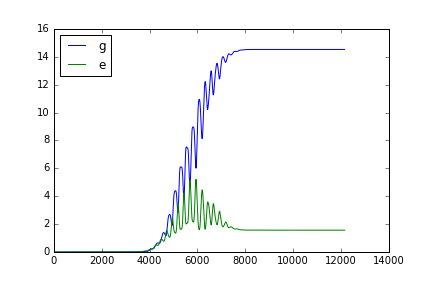
\includegraphics[width=1.0\columnwidth]{warming.png}
   \caption{This is a representative plot of the average value of the ground and excited state vibrational quantum number of a system with S=0.8 and a nonzero $c$, while a laser interacts with it.   The heating is notable in both wells and we'd expect to be able to see signatures of this heating.}
	\label{fig:groundHeating}
\end{figure}

Unfortunately, there is no qualitative difference, here, between the two Figures \ref{fig:cEneg4} and \ref{fig:cEneg1} despite the fact that they are 5 orders of magnitude in $c$ away from each other, so we conclude that there is likely not a way to discriminate between these two situations using IR spectroscopy.  We suspect it would be more fruitful to look into resonance Raman~\cite{ResonanceRaman} as a distinguishing method.

\begin{figure}
   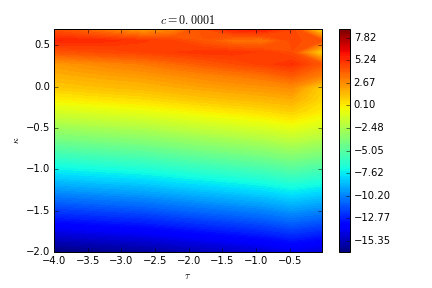
\includegraphics[width=1.0\columnwidth]{0_0001_expProtocol.png}
   \caption{This is a plot of the spectral power at the frequency of the ground vibrational state for $c=0.0001$ as a function of $\tau$ and $\kappa$ for $S=0.8$}
	\label{fig:cEneg4}
\end{figure}


\begin{figure}
   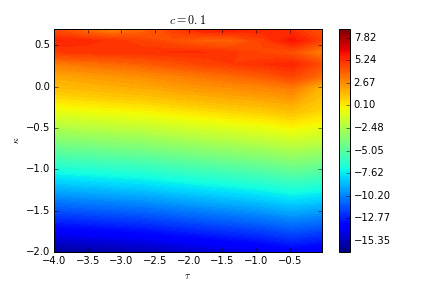
\includegraphics[width=1.0\columnwidth]{0_1_expProtocol.png}
   \caption{This is a plot of the spectral power at the frequency of the ground vibrational state for $c=0.1$ as a function of $\tau$ and $\kappa$ for $S=0.8$}
	\label{fig:cEneg1}
\end{figure}
